% Seminar 1: Randamente și Staționaritate
% Statistica Piețelor Financiare
% Program de licență, Academia de Studii Economice din București

\documentclass[9pt, aspectratio=169, t]{beamer}

% Asigură încadrarea conținutului pe diapozitive
\setbeamersize{text margin left=8mm, text margin right=8mm}

%=============================================================================
% CONFIGURARE TEMĂ ȘI STIL
%=============================================================================
\usetheme{default}

% Color Palette
\definecolor{MainBlue}{RGB}{26, 58, 110}
\definecolor{AccentBlue}{RGB}{26, 58, 110}
\definecolor{IDAred}{RGB}{205, 0, 0}
\definecolor{DarkGray}{RGB}{51, 51, 51}
\definecolor{MediumGray}{RGB}{128, 128, 128}
\definecolor{LightGray}{RGB}{248, 248, 248}
\definecolor{VeryLightGray}{RGB}{235, 235, 235}
\definecolor{KeynoteGray}{RGB}{218, 218, 218}
\definecolor{SectionGray}{RGB}{120, 120, 120}
\definecolor{FooterGray}{RGB}{100, 100, 100}
\definecolor{Crimson}{RGB}{220, 53, 69}
\definecolor{Forest}{RGB}{46, 125, 50}
\definecolor{Amber}{RGB}{181, 133, 63}
\definecolor{Orange}{RGB}{230, 126, 34}
\definecolor{Purple}{RGB}{142, 68, 173}

% Gradient background (background canvas ensures it works on fragile frames too)
\setbeamertemplate{background canvas}{%
    \begin{tikzpicture}[remember picture, overlay]
        \shade[shading=axis, shading angle=315,
        top color=white, bottom color=KeynoteGray]
        (current page.south west) rectangle (current page.north east);
    \end{tikzpicture}%
}

\setbeamercolor{palette primary}{bg=MainBlue, fg=white}
\setbeamercolor{palette secondary}{bg=MainBlue!85, fg=white}
\setbeamercolor{palette tertiary}{bg=MainBlue!70, fg=white}
\setbeamercolor{structure}{fg=MainBlue}
\setbeamercolor{title}{fg=IDAred}
\setbeamercolor{frametitle}{fg=IDAred, bg=}
\setbeamercolor{block title}{bg=MainBlue, fg=white}
\setbeamercolor{block body}{bg=VeryLightGray, fg=DarkGray}
\setbeamercolor{block title alerted}{bg=Crimson, fg=white}
\setbeamercolor{block body alerted}{bg=Crimson!8, fg=DarkGray}
\setbeamercolor{block title example}{bg=Forest, fg=white}
\setbeamercolor{block body example}{bg=Forest!8, fg=DarkGray}
\setbeamercolor{item}{fg=MainBlue}

% Culori subsol
\setbeamercolor{author in head/foot}{fg=FooterGray, bg=}
\setbeamercolor{title in head/foot}{fg=FooterGray, bg=}
\setbeamercolor{date in head/foot}{fg=FooterGray, bg=}
\setbeamercolor{section in head/foot}{fg=FooterGray, bg=}
\setbeamercolor{subsection in head/foot}{fg=FooterGray, bg=}

% Stiluri marcatori
\setbeamertemplate{itemize item}{\color{MainBlue}$\boxdot$}
\setbeamertemplate{itemize subitem}{\color{MainBlue}$\blacktriangleright$}
\setbeamertemplate{itemize subsubitem}{\color{MainBlue}\tiny$\bullet$}
\setbeamertemplate{itemize/enumerate body begin}{\normalsize}
\setbeamertemplate{itemize/enumerate subbody begin}{\normalsize}

% Spațiere elemente
\setlength{\leftmargini}{10pt}
\setlength{\leftmarginii}{10pt}
\makeatletter
\def\@listi{\leftmargin\leftmargini \topsep 0pt \parsep 0pt \itemsep 0pt}
\def\@listii{\leftmargin\leftmarginii \topsep 0pt \parsep 0pt \itemsep 0pt}
\makeatother

\setbeamertemplate{navigation symbols}{}

%=============================================================================
% ANTET PERSONALIZAT
%=============================================================================
\setbeamertemplate{headline}{%
    \vskip10pt%
    \hbox to \paperwidth{%
        \hskip0.5cm%
        {\small\color{FooterGray}\renewcommand{\hyperlink}[2]{##2}\insertsectionhead}%
        \hfill%
        \textcolor{FooterGray}{\small\insertframenumber}%
        \hskip0.5cm%
    }%
    \vskip4pt%
    {\color{FooterGray}\hrule height 0.4pt}%
}

%=============================================================================
% SUBSOL PERSONALIZAT
%=============================================================================
\usepackage{fontawesome5}

\setbeamertemplate{footline}{%
    {\color{FooterGray}\hrule height 0.4pt}%
    \vskip4pt%
    \hbox to \paperwidth{%
        \hskip0.5cm%
        \textcolor{FooterGray}{\small Statistica Piețelor Financiare --- Seminar}%
        \hfill%
        \raisebox{-0.1em}{%
            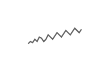
\begin{tikzpicture}[x=0.08em, y=0.08em, line width=0.4pt]
                \draw[FooterGray] (0,3) -- (1,4) -- (2,3.5) -- (3,5) -- (4,4) -- (5,6) -- (6,5.5) -- (7,4) -- (8,5) -- (9,7) -- (10,6) -- (11,5) -- (12,6.5) -- (13,8) -- (14,7) -- (15,6) -- (16,7.5) -- (17,9) -- (18,8) -- (19,7) -- (20,8.5) -- (21,10) -- (22,9) -- (23,8) -- (24,9.5);
            \end{tikzpicture}%
        }%
        \hskip0.5cm%
    }%
    \vskip6pt%
}

%=============================================================================
% PACHETE
%=============================================================================
\usepackage[utf8]{inputenc}
\usepackage[T1]{fontenc}
\usepackage{amsmath, amssymb, amsthm}
\usepackage{mathtools}
\usepackage{bm}
\usepackage{tikz}
\usetikzlibrary{arrows.meta, positioning, shapes, calc, decorations.pathreplacing, shadings}
\usepackage{booktabs}
\usepackage{multirow}
\usepackage{array}
\usepackage{graphicx}
\usepackage{hyperref}
\usepackage{colortbl}
\usepackage{listings}
\lstset{language=Python, basicstyle=\ttfamily\scriptsize, keywordstyle=\color{MainBlue}\bfseries,
  commentstyle=\color{Forest}, stringstyle=\color{Crimson}, breaklines=true,
  frame=none, backgroundcolor=\color{VeryLightGray}, xleftmargin=2mm}
\hypersetup{colorlinks=true, linkcolor=MainBlue, urlcolor=MainBlue}
\graphicspath{{../../logos/}{../../charts/}{../../photos/}}
\hfuzz=2pt
\vfuzz=2pt

%=============================================================================
% COMANDA QUANTLET
%=============================================================================
\newcommand{\quantlet}[2]{%
    \hfill\href{#2}{%
        \raisebox{-0.15em}{
\includegraphics[height=0.7em]{ql_logo.png}}%
        \textcolor{MainBlue}{\tiny\ #1}%
    }%
}

%=============================================================================
% PAGINĂ TITLU PERSONALIZATĂ
%=============================================================================
\defbeamertemplate*{title page}{hybrid}[1][]
{
    \vspace{0.2cm}
    \begin{center}
        \href{https://www.ase.ro}{
\includegraphics[height=1.0cm]{ase_logo.png}}\hspace{0.3cm}%
        \href{https://theida.net}{
\includegraphics[height=1.0cm]{ida_logo.png}}\hspace{0.3cm}%
        \href{https://blockchain-research-center.com}{
\includegraphics[height=1.0cm]{brc_logo.png}}\hspace{0.3cm}%
        \href{https://www.ai4efin.ase.ro}{
\includegraphics[height=1.0cm]{ai4efin_logo.png}}\hspace{0.3cm}%
        \href{https://ipe.ro/new}{
\includegraphics[height=1.0cm]{acad_logo.png}}\hspace{0.3cm}%
        \href{https://www.digital-finance-msca.com}{
\includegraphics[height=1.0cm]{msca_logo.png}}%
    \end{center}

    \vspace{0.6cm}

    \begin{center}
        \begin{minipage}{0.1\textwidth}
            \centering
            \href{https://quantlet.com}{
\includegraphics[height=1.1cm]{ql_logo.png}}
        \end{minipage}%
        \begin{minipage}{0.78\textwidth}
            \centering
            {\LARGE\bfseries\usebeamercolor[fg]{title}\inserttitle}

            \vspace{0.3cm}

            {\usebeamerfont{subtitle}\usebeamercolor[fg]{title}\insertsubtitle}
        \end{minipage}%
        \begin{minipage}{0.1\textwidth}
            \centering
            \href{https://quantinar.com}{
\includegraphics[height=1.1cm]{qr_logo.png}}
        \end{minipage}
    \end{center}

    \vspace{0.6cm}

    \hspace{0.5cm}\begin{minipage}[t]{0.9\textwidth}
        \raggedright{\usebeamerfont{author}\insertauthor}
    \end{minipage}

    \vspace{0.3cm}

    \hspace{0.5cm}\begin{minipage}[t]{0.9\textwidth}
        \raggedright\small\insertinstitute
    \end{minipage}
}

%=============================================================================
% MEDII PENTRU TEOREME
%=============================================================================
\theoremstyle{definition}
\setbeamertemplate{theorems}[numbered]
\newtheorem{defn}{Definiție}
\newtheorem{thm}{Teoremă}
\newtheorem{prop}{Propoziție}
\newtheorem{rmk}{Observație}

%=============================================================================
% CENTRED MINIPAGE
%=============================================================================
\newenvironment{cminipage}[1]{%
    \par\noindent\hfill\begin{minipage}{#1}\ignorespaces
}{%
    \end{minipage}\hfill\null\par
}

%=============================================================================
% COMENZI PERSONALIZATE
%=============================================================================
\newcommand{\E}{\mathbb{E}}
\newcommand{\Var}{\text{Var}}
\newcommand{\Cov}{\text{Cov}}
\newcommand{\Corr}{\text{Corr}}
\newcommand{\R}{\mathbb{R}}
\newcommand{\N}{\mathbb{N}}
\newcommand{\Z}{\mathbb{Z}}
\newcommand{\B}{\mathbf{B}}
\newcommand{\imark}{\textcolor{MainBlue}{\textbullet}}
\newcommand{\RMSE}{\text{RMSE}}
\newcommand{\MAE}{\text{MAE}}
\newcommand{\MAPE}{\text{MAPE}}

%=============================================================================
% INFORMAȚII TITLU
%=============================================================================
\title[Statistica Piețelor Financiare]{Statistica Piețelor Financiare}
\subtitle{Seminar 1: Randamente și Staționaritate}
\author[D.T. Pele, A. Amza]{Daniel Traian PELE \\ Antoaneta Amza}
\institute{Academia de Studii Economice din București\\
IDA Institute Digital Assets\\
Blockchain Research Center\\
AI4EFin Artificial Intelligence for Energy Finance\\
Academia Română, Institutul de Prognoză Economică\\
MSCA Digital Finance}
\date{}

\begin{document}

% Pagina de titlu (fără antet/subsol)
{
\setbeamertemplate{headline}{}
\setbeamertemplate{footline}{}
\begin{frame}
    \titlepage
\end{frame}
}

%=============================================================================
% OBIECTIVE
%=============================================================================
\section{Obiective}

\begin{frame}{Obiective de învățare --- Seminar 1}
\begin{block}{La sfârșitul acestui seminar, veți fi capabili să:}
\begin{enumerate}
    \item[\textcolor{MainBlue}{\textbf{1.}}] \textbf{Calculați} randamente simple și logaritmice din date de preț
    \item[\textcolor{MainBlue}{\textbf{2.}}] \textbf{Comparați} agregarea temporală a celor două tipuri de randamente
    \item[\textcolor{MainBlue}{\textbf{3.}}] \textbf{Explicați} pierderea din varianță (variance drag) și impactul ei
    \item[\textcolor{MainBlue}{\textbf{4.}}] \textbf{Argumentați} de ce analizăm randamente și nu prețuri (staționaritate)
    \item[\textcolor{MainBlue}{\textbf{5.}}] \textbf{Implementați} calculul randamentelor în Python
\end{enumerate}
\end{block}
\vspace{0.2cm}
\begin{center}
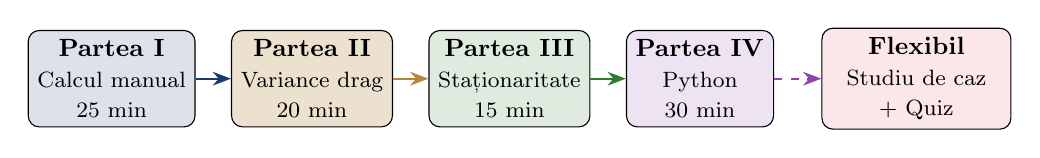
\begin{tikzpicture}[>=Stealth, node distance=0.45cm, every node/.style={font=\small}]
    \node[draw, rounded corners, fill=MainBlue!15, minimum width=1.6cm, minimum height=0.8cm, align=center] (p1) {\textbf{Partea I}\\ \footnotesize Calcul manual\\ \footnotesize 25 min};
    \node[draw, rounded corners, fill=Amber!25, minimum width=1.6cm, minimum height=0.8cm, align=center, right=0.45cm of p1] (p2) {\textbf{Partea II}\\ \footnotesize Variance drag\\ \footnotesize 20 min};
    \node[draw, rounded corners, fill=Forest!15, minimum width=1.6cm, minimum height=0.8cm, align=center, right=0.45cm of p2] (p3) {\textbf{Partea III}\\ \footnotesize Staționaritate\\ \footnotesize 15 min};
    \node[draw, rounded corners, fill=Purple!15, minimum width=1.6cm, minimum height=0.8cm, align=center, right=0.45cm of p3] (p4) {\textbf{Partea IV}\\ \footnotesize Python\\ \footnotesize 30 min};
    \draw[->, thick, MainBlue] (p1) -- (p2);
    \draw[->, thick, Amber] (p2) -- (p3);
    \draw[->, thick, Forest] (p3) -- (p4);
    % Flexible section
    \node[draw, rounded corners, fill=Crimson!12, minimum width=2.4cm, minimum height=0.8cm, align=center, right=0.6cm of p4] (p5) {\textbf{Flexibil}\\ \footnotesize Studiu de caz\\ \footnotesize + Quiz};
    \draw[->, thick, Purple, dashed] (p4) -- (p5);
\end{tikzpicture}

\vspace{0.1cm}
{\footnotesize\textcolor{MediumGray}{Total: 90 min predare + studiu de caz și quiz ca material suplimentar}}
\end{center}
\end{frame}

%=============================================================================
% PARTEA I: CALCUL MANUAL (25 min)
%=============================================================================
\section{Partea I: Calcul manual}

\begin{frame}[shrink=5]{Exercițiul 1: Calcul randamente simple și logaritmice}
\begin{block}{Date de preț}
\begin{center}
{\small\renewcommand{\arraystretch}{1.3}
\begin{tabular}{lcccc}
\toprule
$t$ & 0 & 1 & 2 & 3 \\
\midrule
$P_t$ & 100 & 110 & 99 & 120 \\
\bottomrule
\end{tabular}}
\end{center}
\end{block}
\vspace{0.1cm}
\begin{columns}[T]
\begin{column}{0.48\textwidth}
\begin{exampleblock}{$R_t = \frac{P_t - P_{t-1}}{P_{t-1}}$ (simple)}
\begin{itemize}
    \item $R_1 = 10/100 = \mathbf{+10.00\%}$
    \item $R_2 = -11/110 = \mathbf{-10.00\%}$
    \item $R_3 = 21/99 = \mathbf{+21.21\%}$
\end{itemize}
\end{exampleblock}
\end{column}
\begin{column}{0.48\textwidth}
\begin{exampleblock}{$r_t = \ln(P_t / P_{t-1})$ (logaritmice)}
\begin{itemize}
    \item $r_1 = \ln(1.10) = \mathbf{+9.531\%}$
    \item $r_2 = \ln(0.9\overline{0}) = \mathbf{-10.536\%}$
    \item $r_3 = \ln(1.2121) = \mathbf{+19.237\%}$
\end{itemize}
\end{exampleblock}
\end{column}
\end{columns}
\vspace{0.1cm}
\begin{alertblock}{Observație cheie}
$R_1 + R_2 = 0\%$, dar prețul a scăzut la 99! Randamentele simple \textbf{nu sunt aditive} --- se compun multiplicativ: $\prod(1+R_t)$.
\end{alertblock}
\end{frame}

\begin{frame}[shrink=5]{Exercițiul 1: Aditivitate și comparație}
\begin{columns}[T]
\begin{column}{0.48\textwidth}
\begin{exampleblock}{Verificare: aditivitate log}
\begin{itemize}
    \item $r_1 + r_2 + r_3 = \mathbf{+18.232\%}$
    \item $\ln(P_3/P_0) = \ln(1.20) = \mathbf{+18.232\%}$ \checkmark
\end{itemize}
\end{exampleblock}
\begin{block}{Compunere simplă (multiplicativă)}
\[
\textstyle\prod_{t=1}^{3}(1+R_t) = 1.10 \times 0.90 \times 1.2121 = 1.20
\]
\begin{itemize}
    \item $R_{\text{total}} = 20\%$; \; $e^{r_{\text{total}}} - 1 = 20\%$ \checkmark
\end{itemize}
\end{block}
\end{column}
\begin{column}{0.50\textwidth}
\begin{center}
{\small
\renewcommand{\arraystretch}{1.2}
\begin{tabular}{lcccc}
\toprule
& Per.\ 1 & Per.\ 2 & Per.\ 3 & \textbf{Total} \\
\midrule
$R_t$ & $+10.00$ & $-10.00$ & $+21.21$ & $+20.00$ \\
$r_t$ & $+9.53$ & $-10.54$ & $+19.24$ & $+18.23$ \\
\bottomrule
\end{tabular}
}
\end{center}
\vspace{0.1cm}
{\footnotesize Unitate: \%. Ambele metode $\Rightarrow$ aceeași avere finală.}
\end{column}
\end{columns}
\vspace{0.1cm}
\begin{alertblock}{Concluzie}
\begin{itemize}
    \item Log-randamentele se \textbf{adună}, simplele se \textbf{înmulțesc}
    \item Folosim log-randamente în modelarea statistică pentru aditivitate temporală
\end{itemize}
\end{alertblock}
\end{frame}

\begin{frame}{Vizualizare: Analiza randamentelor (S\&P 500, 2000--2024)}
\begin{center}
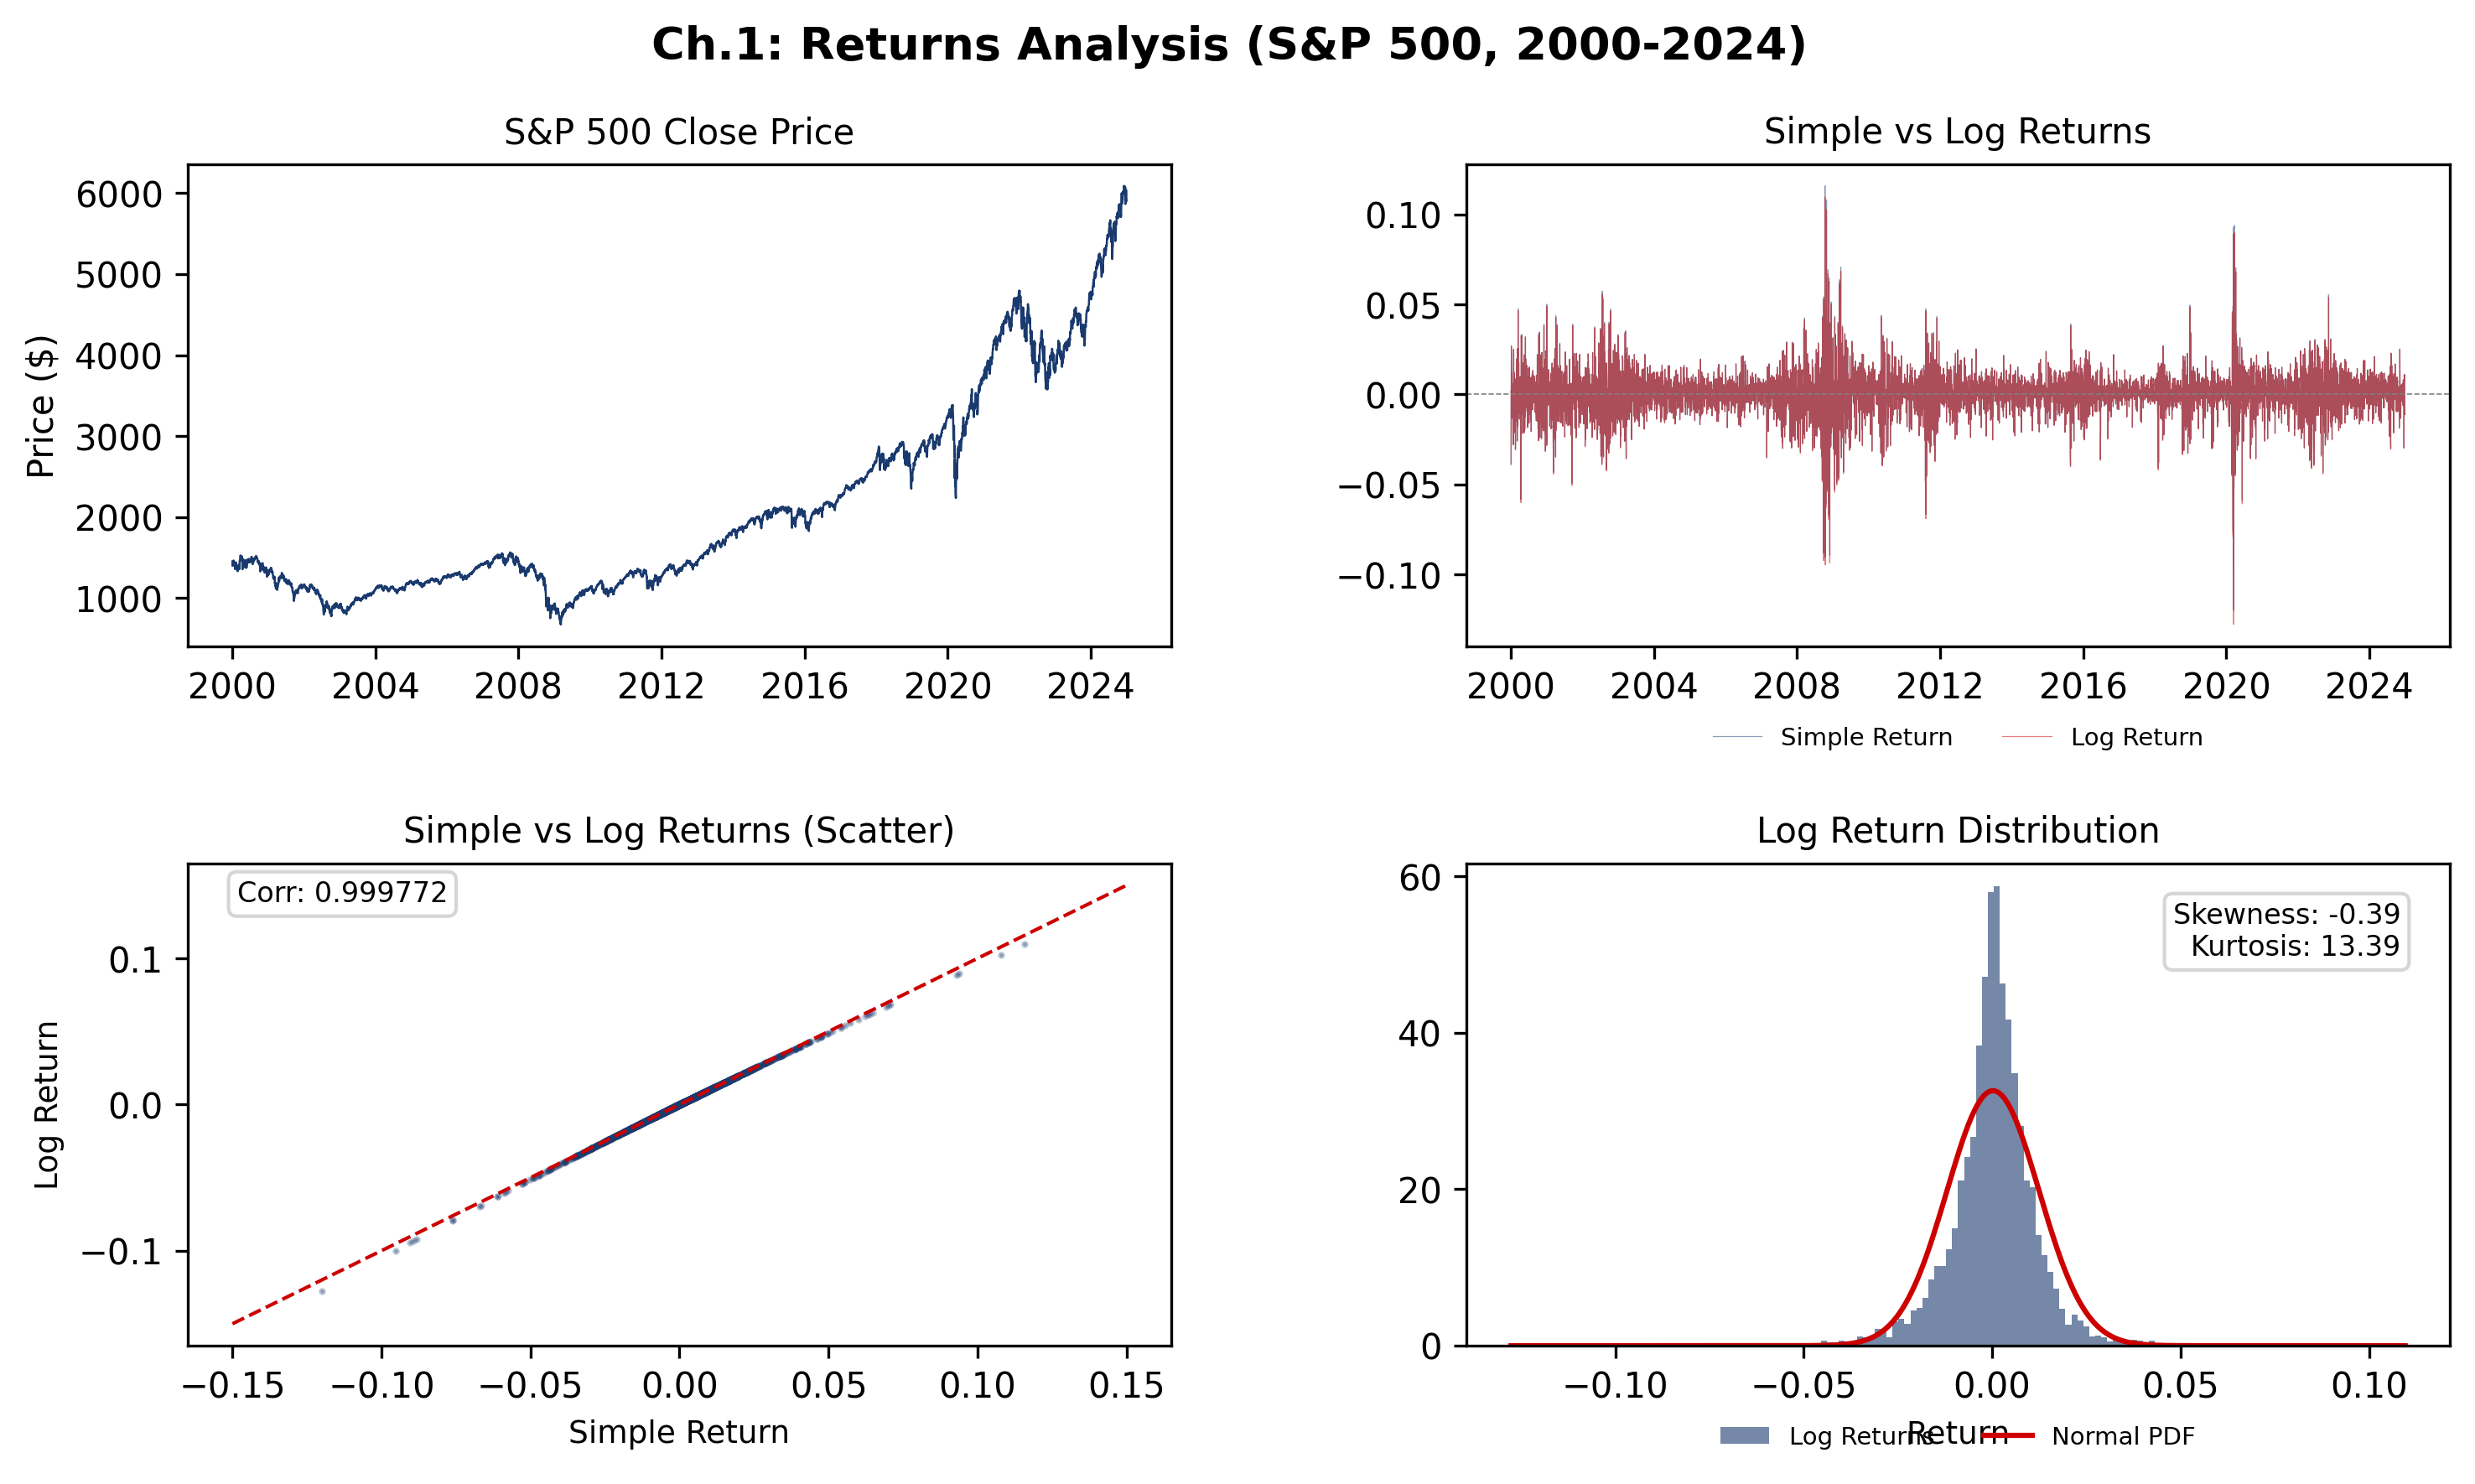
\includegraphics[width=0.62\linewidth]{sfm_ch1_returns_sp500.png}
\end{center}
\vspace{-0.3cm}
\begin{itemize}
    \item \textbf{Scatter}: corelație $\approx 0.9998$ între $R_t$ și $r_t$ --- aproape identice pentru valori mici
    \item \textbf{Histogramă}: cozi mai groase decât Normala ($K = 13.4$, $S = -0.39$)
\end{itemize}
\quantlet{SFM\_ch1\_returns}{https://github.com/QuantLet/Stat_fin_markets/tree/master/Ch_01/SFM_ch1_returns}
\end{frame}

\section{De la calcul la intuiție}

\begin{frame}{Sondaj rapid --- Votați acum!}
\begin{alertblock}{\faIcon{poll} Întrebare}
\begin{itemize}
    \item Investiți \textbf{\$100} într-un activ. Acesta crește cu $+50\%$ într-un an, apoi scade cu $-50\%$ în anul următor.
    \item \textbf{Cu cât rămâneți?}
\end{itemize}
\end{alertblock}
\vspace{0.5cm}
\begin{columns}[T]
\begin{column}{0.24\textwidth}
\begin{center}
\tikz\node[draw, rounded corners, fill=MainBlue!15, minimum width=2.5cm, minimum height=1.2cm, align=center] {\textbf{A)}\\ \$100\\ (0\% net)};
\end{center}
\end{column}
\begin{column}{0.24\textwidth}
\begin{center}
\tikz\node[draw, rounded corners, fill=Amber!25, minimum width=2.5cm, minimum height=1.2cm, align=center] {\textbf{B)}\\ \$90\\ ($-10\%$)};
\end{center}
\end{column}
\begin{column}{0.24\textwidth}
\begin{center}
\tikz\node[draw, rounded corners, fill=Crimson!15, minimum width=2.5cm, minimum height=1.2cm, align=center] {\textbf{C)}\\ \$75\\ ($-25\%$)};
\end{center}
\end{column}
\begin{column}{0.24\textwidth}
\begin{center}
\tikz\node[draw, rounded corners, fill=Forest!15, minimum width=2.5cm, minimum height=1.2cm, align=center] {\textbf{D)}\\ \$50\\ ($-50\%$)};
\end{center}
\end{column}
\end{columns}
\end{frame}

\begin{frame}{Sondaj rapid --- Răspuns}
\begin{exampleblock}{Calcul}
\begin{itemize}
    \item \$100 $\times$ 1.50 $=$ \$150, apoi \$150 $\times$ 0.50 $=$ \textcolor{Crimson}{\textbf{\$75}}
    \item Pierdeți \textbf{25\%}, nu 0\%!
\end{itemize}
\end{exampleblock}
\vspace{0.3cm}
\begin{alertblock}{De ce?}
\begin{itemize}
    \item Creșterea de 50\% se aplică pe \$100, dar scăderea de 50\% se aplică pe \$150 --- o \textit{bază mai mare}
    \item Acesta este \textbf{variance drag} în acțiune: volatilitatea \textit{distruge} averea
    \item Formula: pierdere $\approx \sigma^2 / 2$ pe an (vom demonstra în Partea II)
\end{itemize}
\end{alertblock}
\end{frame}

\begin{frame}[shrink=3]{Discuție ghidată: De ce $+50\%$ și $-50\%$ nu se anulează?}
\begin{alertblock}{Tocmai ați văzut: \$100 → \$150 → \$75. Dar cum arată cu log-randamente?}
\end{alertblock}
\vspace{0.2cm}
\begin{columns}[T]
\begin{column}{0.48\textwidth}
\begin{block}{Randamente simple (multiplicative)}
\[
(1.50)(0.50) = 0.75 \neq 1.00
\]
\begin{itemize}
    \item $R_1 + R_2 = +50\% + (-50\%) = 0\%$
    \item Dar averea finală: \$75, nu \$100!
    \item Randamentele simple \textbf{nu} sunt aditive
\end{itemize}
\end{block}
\end{column}
\begin{column}{0.48\textwidth}
\begin{exampleblock}{Randamente log (aditive)}
\[
r_{\text{up}} = \ln(1.50) = +40.55\%
\]
\[
r_{\text{down}} = \ln(0.50) = -69.31\%
\]
\begin{itemize}
    \item Suma: $-28.77\% = \ln(0.75)$ \checkmark
    \item Log-randamentele reflectă \textbf{corect} pierderea
\end{itemize}
\end{exampleblock}
\end{column}
\end{columns}
\vspace{0.2cm}
\begin{alertblock}{Mesaj cheie}
\begin{itemize}
    \item Asimetria este dramatică: trebuie $+100\%$ ca să recuperezi $-50\%$
    \item Cu cât volatilitatea e mai mare, cu atât pierderea e mai severă
\end{itemize}
\end{alertblock}
\end{frame}

%=============================================================================
% PARTEA II: VARIANCE DRAG (20 min)
%=============================================================================
\section{Partea II: Variance Drag}

\begin{frame}{Variance Drag: Formulă și intuiție}
\begin{defn}[Pierderea din varianță]
\begin{itemize}
    \item Relația dintre randamentul aritmetic așteptat și cel geometric:
    \[
    \E[r] \approx \E[R] - \frac{1}{2}\sigma^2
    \]
    \item $\E[R]$ --- randamentul simplu așteptat
    \item $\E[r]$ --- randamentul logaritmic așteptat
    \item $\sigma^2$ --- varianța randamentelor simple
\end{itemize}
\end{defn}
\vspace{0.2cm}
\begin{itemize}
    \item Pierderea din varianță crește \textbf{cvadratic} cu volatilitatea: dublarea $\sigma$ $\Rightarrow$ cvadruplarea pierderii
    \item Aceasta este o consecință a \textbf{inegalității lui Jensen}: $\E[\ln(1+R)] < \ln(1+\E[R])$ deoarece $\ln$ este concavă.
    \item \textbf{Implicație}: volatilitatea \textit{distruge} averea pe termen lung, chiar dacă randamentul aritmetic este pozitiv.
\end{itemize}
\end{frame}

\begin{frame}[shrink=7]{Exercițiul 2: Două active, aceeași medie, volatilitate diferită}
\begin{block}{Enunț}
\begin{center}
{\small
\renewcommand{\arraystretch}{1.3}
\begin{tabular}{lccc}
\toprule
\textbf{Activ} & $\E[R]$ & $\sigma$ & $\E[r] \approx \E[R] - \sigma^2/2$ \\
\midrule
A & 12\% & 10\% & ? \\
B & 12\% & 30\% & ? \\
\bottomrule
\end{tabular}
}
\end{center}
\end{block}
\vspace{0.2cm}
\begin{exampleblock}{Rezolvare}
\begin{itemize}
    \item \textbf{Activ A}: $\E[r]_A \approx 0.12 - 0.5 \times (0.10)^2 = 0.12 - 0.005 = \mathbf{11.50\%}$
    \item \textbf{Activ B}: $\E[r]_B \approx 0.12 - 0.5 \times (0.30)^2 = 0.12 - 0.045 = \mathbf{7.50\%}$
\end{itemize}
\end{exampleblock}
\vspace{0.1cm}
\begin{alertblock}{Întrebare pentru studenți}
\begin{itemize}
    \item Care activ produce mai multă avere pe termen lung?
    \item Calculați $W_{10}$ pentru ambele ($W_0 = 1$)
\end{itemize}
\end{alertblock}
\end{frame}

\begin{frame}[shrink=6]{Exercițiul 2: Rezolvare --- Averea pe termen lung}
\begin{columns}[T]
\begin{column}{0.52\textwidth}
\begin{block}{$W_T = W_0 \cdot e^{T \times \E[r]}$}
\begin{itemize}
    \item \textbf{A}: $W_{10} = e^{10 \times 0.115} = \mathbf{3.16}$ (triplare)
    \item \textbf{B}: $W_{10} = e^{10 \times 0.075} = \mathbf{2.12}$ (dublare)
\end{itemize}
\end{block}
\vspace{0.05cm}
{\small
\renewcommand{\arraystretch}{1.1}
\begin{tabular}{lcccc}
\toprule
\textbf{Activ} & $\E[R]$ & $\sigma$ & $\E[r]$ & $W_{10}$ \\
\midrule
A & 12\% & 10\% & 11.50\% & \textcolor{Forest}{\textbf{3.16}} \\
B & 12\% & 30\% & 7.50\% & \textcolor{Crimson}{\textbf{2.12}} \\
\bottomrule
\end{tabular}
}
\end{column}
\begin{column}{0.46\textwidth}
\begin{center}
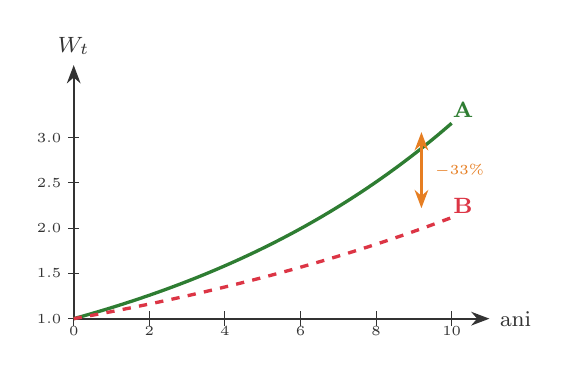
\begin{tikzpicture}[x=0.48cm, y=1.15cm, >=Stealth]
    % Axes: y scale = 1.15cm per unit of W (linear, W from 1 to 3.5)
    \draw[->, thick, DarkGray] (0,0) -- (11,0) node[right] {\footnotesize ani};
    \draw[->, thick, DarkGray] (0,0) -- (0,2.8) node[above] {\footnotesize $W_t$};
    % Y-axis labels (linear: y = (W - 1) in scaled units)
    \foreach \w in {1.0, 1.5, 2.0, 2.5, 3.0} {
        \pgfmathsetmacro{\ypos}{\w - 1.0}
        \draw[DarkGray] (-0.15,\ypos) -- (0.15,\ypos) node[left=3pt] {\tiny \w};
    }
    % X-axis labels
    \foreach \x in {0,2,4,6,8,10} {
        \draw[DarkGray] (\x,-0.08) -- (\x,0.08) node[below=2pt] {\tiny \x};
    }
    % Curve A: W = e^{0.115*t}, plotted as y = e^{0.115*t} - 1
    \draw[Forest, very thick] plot[smooth, domain=0:10, samples=30]
        (\x, {exp(0.115*\x) - 1});
    % Curve B: W = e^{0.075*t}, plotted as y = e^{0.075*t} - 1
    \draw[Crimson, very thick, dashed] plot[smooth, domain=0:10, samples=30]
        (\x, {exp(0.075*\x) - 1});
    % End labels
    \node[Forest, font=\footnotesize\bfseries] at (10.3, 2.3) {A};
    \node[Crimson, font=\footnotesize\bfseries] at (10.3, 1.25) {B};
    % Gap annotation
    \draw[<->, thick, Orange] (9.2, 1.22) -- (9.2, 2.06);
    \node[Orange, font=\tiny, right] at (9.3, 1.64) {$-$33\%};
\end{tikzpicture}
\end{center}
\end{column}
\end{columns}
\vspace{0.1cm}
\begin{alertblock}{Concluzie cheie}
\begin{itemize}
    \item \textbf{Volatilitatea mare distruge averea!} Activul B are drag de 4.5\%/an --- pe 10 ani, costă $\approx$33\% din avere
    \item \textit{``Volatility is the cost of uncertainty.''}
\end{itemize}
\end{alertblock}
\end{frame}

\begin{frame}[shrink=7]{Exercițiile 3--5}
\begin{block}{Exercițiul 3: Aditivitatea log-randamentelor --- Arătați că $r_{0,T} = \ln(P_T/P_0) = \sum_{t=1}^{T} r_t$}
\textit{Indiciu}: scrieți $\dfrac{P_T}{P_0} = \dfrac{P_1}{P_0} \cdot \dfrac{P_2}{P_1} \cdots \dfrac{P_T}{P_{T-1}}$ și aplicați $\ln$ pe produs.
\end{block}
\vspace{0.2cm}
\begin{block}{Exercițiul 4: Variance drag --- Arătați că $\E[r] \approx \E[R] - \frac{1}{2}\sigma^2$}
Folosind dezvoltarea Taylor: $\ln(1+R) \approx R - R^2/2$, aplicați $\E[\cdot]$ pe ambii membri.

\textit{Indiciu}: $\E[R^2] = \Var(R) + (\E[R])^2 \approx \sigma^2$ pentru $\E[R] \approx 0$.
\end{block}
\vspace{0.2cm}
\begin{exampleblock}{Exercițiul 5: Inegalitatea lui Jensen --- Deduceți că $\E[\ln(1+R)] \leq \ln(1 + \E[R])$}
Funcția $f(x) = \ln(x)$ este concavă. Enunțați inegalitatea lui Jensen și interpretați: ce implică aceasta pentru relația dintre randamentul geometric și cel aritmetic?
\end{exampleblock}
\end{frame}

\begin{frame}[shrink=7]{Exercițiile 3--5: Soluții}
\begin{exampleblock}{Soluție Ex.\ 3 --- Aditivitate}
$\dfrac{P_T}{P_0} = \displaystyle\prod_{t=1}^{T} \dfrac{P_t}{P_{t-1}} \;\;\Rightarrow\;\; \ln\!\left(\dfrac{P_T}{P_0}\right) = \displaystyle\sum_{t=1}^{T} \underbrace{\ln\!\left(\dfrac{P_t}{P_{t-1}}\right)}_{= \, r_t} \qquad \square$
\end{exampleblock}
\vspace{0.2cm}
\begin{exampleblock}{Soluție Ex.\ 4 --- Variance drag}
$r = \ln(1+R) \approx R - \tfrac{R^2}{2}$. Aplicăm $\E[\cdot]$:
$\E[r] \approx \E[R] - \tfrac{1}{2}\E[R^2] = \E[R] - \tfrac{1}{2}\bigl(\sigma^2 + \mu^2\bigr) \approx \E[R] - \tfrac{1}{2}\sigma^2$ \quad (deoarece $\mu^2 \ll \sigma^2$) $\;\square$
\end{exampleblock}
\vspace{0.2cm}
\begin{exampleblock}{Soluție Ex.\ 5 --- Jensen}
\begin{itemize}
    \item Inegalitatea lui Jensen: dacă $f$ concavă, atunci $\E[f(X)] \leq f(\E[X])$
    \item Cu $f = \ln$, $X = 1+R$: $\;\E[\ln(1+R)] \leq \ln(1+\E[R])$
    \item Interpretare: randamentul geometric $<$ randamentul aritmetic; diferența crește cu $\sigma$ $\;\square$
\end{itemize}
\end{exampleblock}
\end{frame}

%=============================================================================
% PARTEA III: STAȚIONARITATE (15 min)
%=============================================================================
\section{Partea III: Staționaritate}

\begin{frame}[shrink=10]{De ce lucrăm cu randamente, nu cu prețuri?}
\begin{columns}[T]
\begin{column}{0.48\textwidth}
\begin{alertblock}{Prețuri: $P_t \sim I(1)$}
\begin{itemize}
    \item $\E[P_t]$, $\Var(P_t)$ \textbf{nu} sunt constante
    \item Regresia pe prețuri $\Rightarrow$ \textbf{regresie falsă} (Granger \& Newbold, 1974)
\end{itemize}
\end{alertblock}
\end{column}
\begin{column}{0.48\textwidth}
\begin{exampleblock}{Randamente: $r_t \sim I(0)$}
\begin{itemize}
    \item Aproximativ staționare (medie $\approx 0$, varianță $\approx$ ct.)
    \item Metodele statistice sunt \textbf{valide}
\end{itemize}
\end{exampleblock}
\end{column}
\end{columns}
\vspace{0.1cm}
\begin{defn}[Staționaritate slabă (covariance stationarity)]
Un proces $\{X_t\}$ este slab staționar dacă, $\forall\, t, h$:
\[
\E[X_t] = \mu, \qquad \Var(X_t) = \sigma^2 < \infty, \qquad \Cov(X_t, X_{t+h}) = \gamma(h).
\]
\end{defn}
\vspace{0.1cm}
\begin{block}{Consecință}
\begin{itemize}
    \item $P_t \sim I(1)$: nestaționară (rădăcină unitară)
    \item $r_t = \Delta \ln P_t \sim I(0)$: staționară
    \item Metodele clasice (OLS, teste $t$, $F$) \textbf{cer staționaritate}; pe serii $I(1)$ produc rezultate false
\end{itemize}
\end{block}
\end{frame}


\begin{frame}[shrink=7]{Random walk și non-staționaritate}
\begin{block}{Random walk: $P_t = P_{t-1} + \varepsilon_t$, \quad $\varepsilon_t \overset{iid}{\sim} (0, \sigma^2)$}
\end{block}
\begin{columns}[T]
\begin{column}{0.50\textwidth}
\begin{alertblock}{De ce $P_t$ nu e staționară?}
\begin{itemize}
    \item Iterând: $P_t = P_0 + \sum_{s=1}^{t} \varepsilon_s$
    \item $\Var(P_t) = t\,\sigma^2 \;\xrightarrow{t\to\infty}\; \infty$
    \item Varianța \textbf{crește liniar} cu $t$
\end{itemize}
\end{alertblock}
\end{column}
\begin{column}{0.48\textwidth}
\begin{exampleblock}{Dar $r_t = \Delta \ln P_t$ e staționară}
\begin{itemize}
    \item $\E[r_t] = \mu$ (constantă)
    \item $\Var(r_t) = \sigma^2$ (constantă)
    \item $\Cov(r_t, r_{t+h}) = \gamma(h)$ --- doar de $h$
\end{itemize}
\end{exampleblock}
\end{column}
\end{columns}
\vspace{0.1cm}
\begin{block}{Strictă vs.\ slabă}
\begin{itemize}
    \item \textbf{Strictă}: distribuția conjunctă $(X_{t_1}, \ldots, X_{t_k})$ invariantă la translații în timp
    \item \textbf{Slabă}: doar primele două momente invariante (suficient pentru OLS, ACF)
    \item Strictă $\Rightarrow$ slabă (dacă $\E[X_t^2] < \infty$), dar \textbf{nu} reciproc
\end{itemize}
\end{block}
\end{frame}

\begin{frame}[shrink=5]{Regresie falsă: Prețul Amazon vs.\ Abonații Netflix (2010--2020)}
\begin{center}
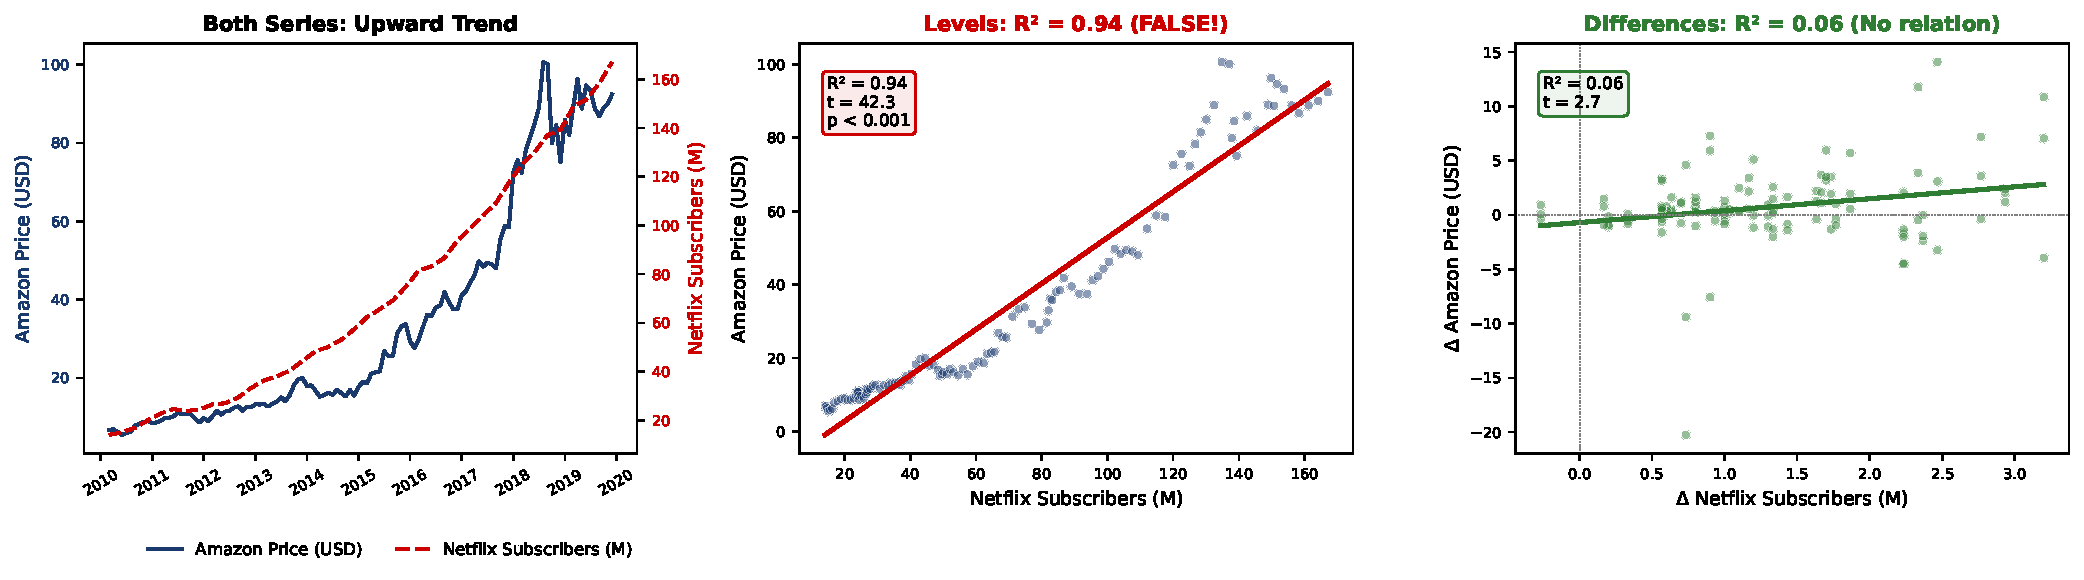
\includegraphics[width=0.88\linewidth]{sfm_ch1_spurious_regression.pdf}
\end{center}
\vspace{-0.3cm}
\begin{columns}[T]
\begin{column}{0.48\textwidth}
\begin{alertblock}{Pe niveluri (preț vs.\ abonați)}
\begin{center}
{\footnotesize
\renewcommand{\arraystretch}{1.1}
\begin{tabular}{lc}
\toprule
$R^2$ & \textbf{0.94} \\
$\hat{\beta}$ & 0.63 \\
$t$-stat & 42.3 \\
\midrule
\textbf{Concluzie} & \textcolor{Crimson}{\textbf{Falsă!}} \\
\bottomrule
\end{tabular}
}
\end{center}
\end{alertblock}
\end{column}
\begin{column}{0.48\textwidth}
\begin{exampleblock}{Pe diferențe ($\Delta P_t$ vs.\ $\Delta S_t$)}
\begin{center}
{\footnotesize
\renewcommand{\arraystretch}{1.1}
\begin{tabular}{lc}
\toprule
$R^2$ & \textbf{0.06} \\
$\hat{\beta}$ & 1.10 \\
$t$-stat & 2.7 \\
\midrule
\textbf{Concluzie} & \textcolor{Forest}{\textbf{Nicio relație}} \\
\bottomrule
\end{tabular}
}
\end{center}
\end{exampleblock}
\end{column}
\end{columns}
\vspace{0.1cm}
{\small \textbf{Lecție}: Un preț de acțiune și un număr de abonați --- variabile \textbf{complet diferite}, dar ambele cu trend $\Rightarrow$ $R^2 = 0.94$ (Granger \& Newbold, 1974). Pe diferențe: $R^2 = 0.06$.}
\quantlet{SFM\_ch1\_stationarity}{https://github.com/QuantLet/Stat_fin_markets/tree/master/Ch_01/SFM_ch1_stationarity}
\end{frame}

%=============================================================================
% PARTEA IV: IMPLEMENTARE PYTHON (30 min) --- total 90 min
%=============================================================================
\section{Partea IV: Implementare Python}

\begin{frame}[fragile]{Implementare Python: Descărcare și calcul}
\begin{block}{Descărcare date + randamente + statistici descriptive}
\begin{lstlisting}
import yfinance as yf
import numpy as np
import matplotlib.pyplot as plt
from statsmodels.tsa.stattools import adfuller
from scipy.stats import jarque_bera

ticker = "AAPL"
data = yf.download(ticker, start="2020-01-01", end="2024-01-01")
data['log_ret'] = np.log(data['Close'] / data['Close'].shift(1))
data['simple_ret'] = data['Close'].pct_change()
r = data['log_ret'].dropna()

print(f"Media zilnica:  {r.mean():.6f}")
print(f"Vol anualizata: {r.std() * np.sqrt(252):.4f}")
print(f"Skewness:       {r.skew():.4f}")
print(f"Kurtosis:       {r.kurtosis() + 3:.4f}")  # scipy: excess
\end{lstlisting}
\end{block}
\quantlet{SFM\_ch1\_returns}{https://github.com/QuantLet/Stat_fin_markets/tree/master/Ch_01/SFM_ch1_returns}
\end{frame}

\begin{frame}[fragile]{Implementare Python: Teste statistice}
\begin{block}{Testul ADF (staționaritate) și Jarque-Bera (normalitate)}
\begin{lstlisting}
# Testul ADF pe log-preturi vs. randamente
adf_price = adfuller(np.log(data['Close'].dropna()))
adf_ret   = adfuller(r)
print(f"ADF log-pret:   stat={adf_price[0]:.3f}, p={adf_price[1]:.4f}")
print(f"ADF randamente: stat={adf_ret[0]:.3f},   p={adf_ret[1]:.4f}")

# Testul Jarque-Bera
jb_stat, jb_p = jarque_bera(r)
print(f"\nJarque-Bera: JB={jb_stat:.1f}, p-value={jb_p:.2e}")

# ACF pe r_t si r_t^2
from statsmodels.tsa.stattools import acf
acf_r  = acf(r, nlags=30)
acf_r2 = acf(r**2, nlags=30)
\end{lstlisting}
\end{block}
{\small
\begin{itemize}
    \item \texttt{adfuller} returnează: (statistic, p-value, lags, nobs, critical values)
    \item $p < 0.05$ $\Rightarrow$ respingem $H_0$ de rădăcină unitară
\end{itemize}}
\quantlet{SFM\_ch1\_stationarity}{https://github.com/QuantLet/Stat_fin_markets/tree/master/Ch_01/SFM_ch1_stationarity}
\end{frame}

\begin{frame}[shrink=5]{Exercițiu AI (I): Prompt Engineering}
\begin{block}{Cerință}
\begin{itemize}
    \item Formulați un prompt către un LLM (ChatGPT, Claude etc.) care să rezolve \textbf{complet} Exercițiul 1 din acest seminar
    \item Promptul trebuie să conțină: datele de intrare, formulele cerute, formatul de output dorit
\end{itemize}
\end{block}
\vspace{0.1cm}
\begin{exampleblock}{Exemplu de prompt bun}
\begin{itemize}
    \item \textit{``Am prețurile de închidere $P_0=100$, $P_1=110$, $P_2=99$, $P_3=120$. Calculează randamentele simple $R_t$ și logaritmice $r_t$ pentru fiecare perioadă. Verifică aditivitatea log-randamentelor. Prezintă rezultatele într-un tabel.''}
\end{itemize}
\end{exampleblock}
\vspace{0.1cm}
\begin{alertblock}{Întrebări de reflecție}
\begin{itemize}
    \item Răspunsul AI este corect matematic? Verificați cu calculul manual
    \item Ce se întâmplă dacă schimbați formularea? Obțineți alt rezultat?
    \item AI-ul a explicat \textbf{de ce} log-randamentele sunt aditive?
\end{itemize}
\end{alertblock}
\end{frame}

\begin{frame}[fragile, shrink=3]{Exercițiu AI (II): Generare și Verificare Cod Python}
\begin{block}{Cerință}
\begin{itemize}
    \item Cereți unui LLM: \textit{``Scrie cod Python care descarcă date AAPL pe 2020--2024, calculează randamente log, verifică staționaritatea cu testul ADF și afișează un grafic preț vs.\ randamente.''}
    \item Rulați codul generat --- funcționează \textit{as-is}?
\end{itemize}
\end{block}
\vspace{0.1cm}
\begin{alertblock}{Checklist de verificare}
\begin{itemize}
    \item Importurile sunt corecte? (yfinance, numpy, statsmodels)
    \item Formula randamentelor: \texttt{np.log(P/P.shift(1))} sau \texttt{pct\_change()}?
    \begin{itemize}
        \item Atenție: \texttt{pct\_change()} $=$ randamente \textbf{simple}, nu log!
    \end{itemize}
    \item Testul ADF: interpretarea corectă a $p$-value?
    \item Graficul are titluri, axe etichetate, legendă?
\end{itemize}
\end{alertblock}
\vspace{0.1cm}
\begin{exampleblock}{Obiectiv pedagogic}
\begin{itemize}
    \item AI-ul este un \textbf{instrument}, nu un înlocuitor --- codul generat trebuie \textbf{întotdeauna verificat}
    \item Eroarea tipică: confuzia între randamente simple și logaritmice
\end{itemize}
\end{exampleblock}
\end{frame}

\begin{frame}{Discuție pe baza graficelor}
\begin{alertblock}{Întrebări pentru studenți --- analizând graficele generate}
\begin{enumerate}
    \item Care serie pare \textbf{staționară}? Care nu? De ce?
    \item Unde observați \textbf{volatility clustering} (gruparea volatilității)?
    \begin{itemize}
        \item Indiciu: priviți perioada martie 2020 (COVID-19).
    \end{itemize}
    \item Sunt randamentele mari urmate de randamente mari (de orice semn)?
    \item Există perioade vizibil ``calme'' alternând cu cele ``agitate''?
\end{enumerate}
\end{alertblock}
\vspace{0.1cm}
\begin{exampleblock}{Fapte stilizate observabile vizual}
\begin{itemize}
    \item \textbf{Clustering}: perioadele volatile vin în grupuri
    \item \textbf{Cozi groase}: câteva randamente extreme (departe de medie)
    \item \textbf{Medie $\approx 0$}: randamentele fluctuează în jurul zero-ului
    \item Acestea sunt \textbf{faptele stilizate} ale randamentelor financiare (Cont, 2001)
\end{itemize}
\end{exampleblock}
\end{frame}

%=============================================================================
% STUDIU DE CAZ: S&P 500
%=============================================================================
\section{Studiu de caz: S\&P 500}

\begin{frame}{Studiu de caz: S\&P 500 --- Preț vs.\ Randamente}
\begin{columns}[T]
\begin{column}{0.55\textwidth}
\begin{center}
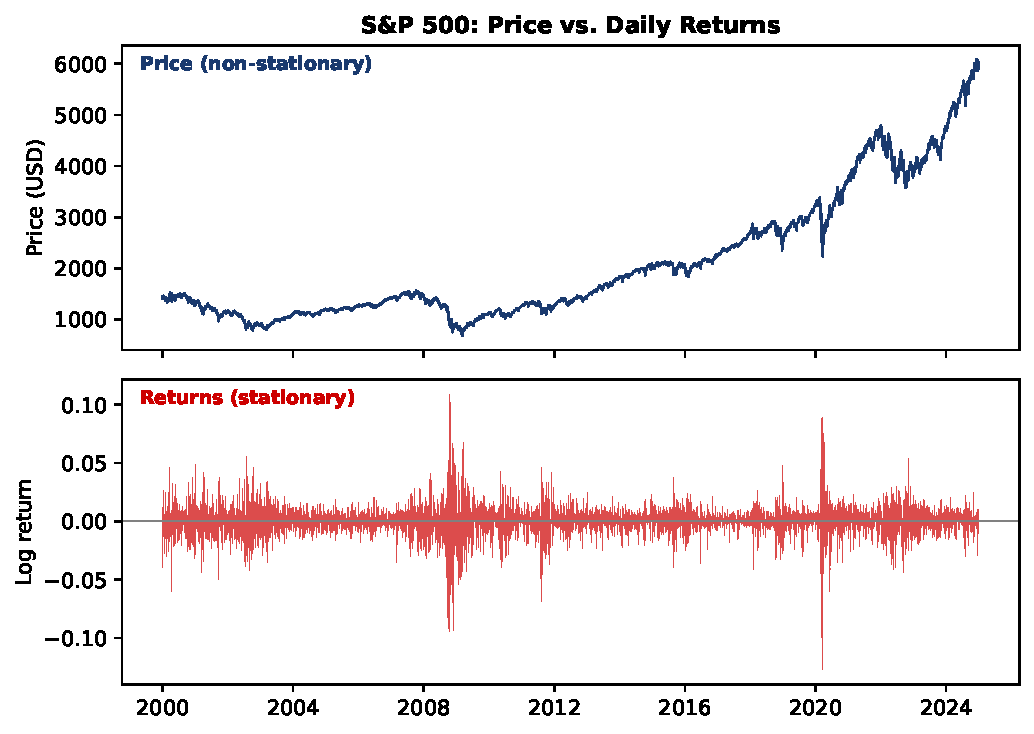
\includegraphics[width=\linewidth]{sfm_ch1_stationarity.pdf}
\end{center}
\end{column}
\begin{column}{0.43\textwidth}
\begin{block}{Date utilizate}
\begin{itemize}
    \item Indicele S\&P 500
    \item Perioada: 2000--2024
    \item Frecvență: zilnică
\end{itemize}
\end{block}
\vspace{0.05cm}
\begin{exampleblock}{Ce observăm?}
\begin{itemize}
    \item Prețul: trend ascendent, crizele 2008 și 2020 vizibile
    \item Randamentele: oscilează în jurul lui zero
    \item Volatility clustering evident în perioadele de criză
\end{itemize}
\end{exampleblock}
\end{column}
\end{columns}
\quantlet{SFM\_ch1\_stationarity}{https://github.com/QuantLet/Stat_fin_markets/tree/master/Ch_01/SFM_ch1_stationarity}
\end{frame}

\begin{frame}[shrink=3]{Studiu de caz: S\&P 500 --- Testul ADF}
\begin{center}
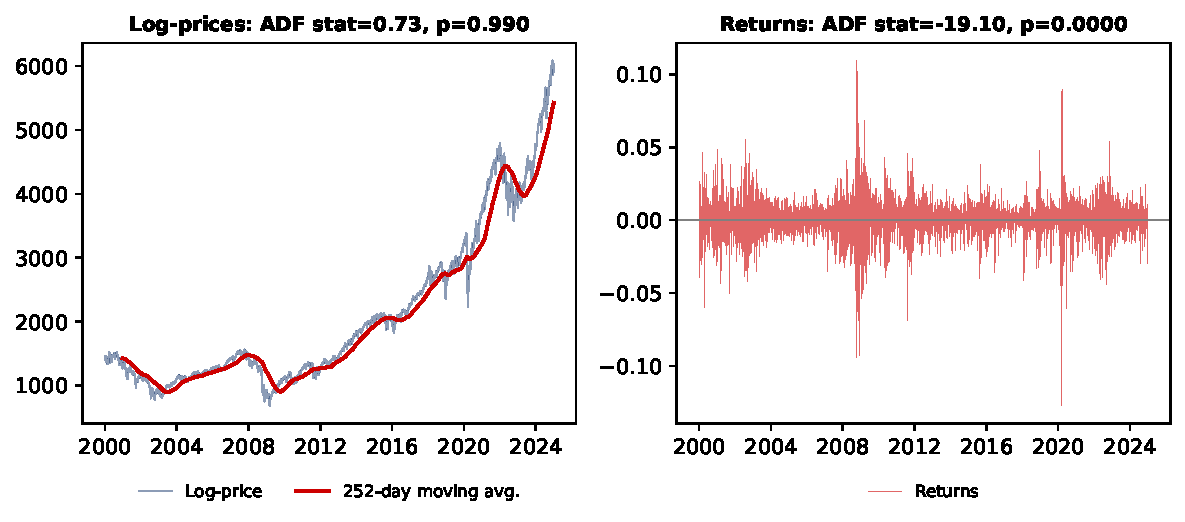
\includegraphics[width=0.72\linewidth]{sfm_ch1_adf_test.pdf}
\end{center}
\vspace{-0.2cm}
\begin{columns}[T]
\begin{column}{0.48\textwidth}
\begin{alertblock}{Log-prețuri}
\begin{itemize}
    \item $H_0$ \textbf{nu} se respinge ($p = 0.98$)
    \item Serie nestaționară, $I(1)$
    \item Rădăcină unitară confirmată
\end{itemize}
\end{alertblock}
\end{column}
\begin{column}{0.48\textwidth}
\begin{exampleblock}{Log-randamente}
\begin{itemize}
    \item $H_0$ se respinge la 1\% ($p \approx 0$)
    \item Serie staționară, $I(0)$
    \item Metodele statistice sunt valide
\end{itemize}
\end{exampleblock}
\end{column}
\end{columns}
\quantlet{SFM\_ch1\_stationarity}{https://github.com/QuantLet/Stat_fin_markets/tree/master/Ch_01/SFM_ch1_stationarity}
\end{frame}

\begin{frame}[shrink=3]{Studiu de caz: ACF --- Randamente vs.\ Randamente pătratice}
\begin{center}
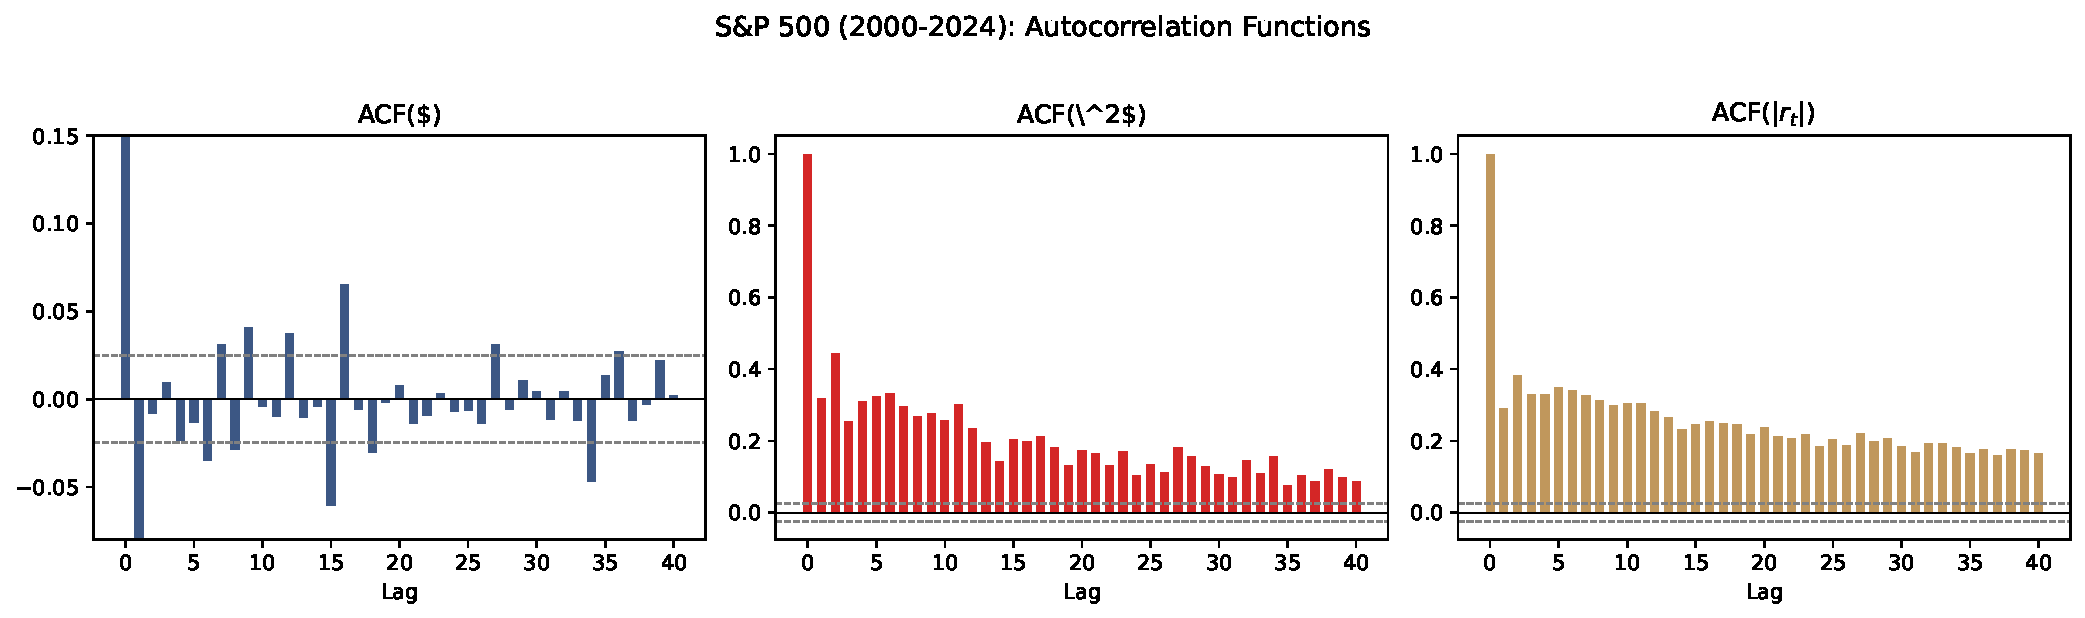
\includegraphics[width=0.82\linewidth]{sfm_ch1_acf_returns.pdf}
\end{center}
\vspace{-0.3cm}
\begin{columns}[T]
\begin{column}{0.48\textwidth}
\begin{exampleblock}{ACF($r_t$) $\approx$ 0}
\begin{itemize}
    \item Randamentele \textbf{nu} sunt autocorelate
    \item Consistent cu ipoteza de piață eficientă (EMH)
    \item Nu putem prezice $r_{t+1}$ din $r_t$
\end{itemize}
\end{exampleblock}
\end{column}
\begin{column}{0.48\textwidth}
\begin{alertblock}{ACF($r_t^2$) $\neq$ 0 --- declin lent}
\begin{itemize}
    \item \textbf{Volatility clustering}: perioadele volatile persistă
    \item Faptul stilizat \#1 (Cont, 2001)
    \item Motivația modelelor GARCH: $\sigma_t^2$ depinde de $r_{t-1}^2$
\end{itemize}
\end{alertblock}
\end{column}
\end{columns}
\vspace{0.1cm}
\begin{itemize}
    \item[\faIcon{exclamation-triangle}] Randamentele sunt necorelate dar \textbf{nu} independente --- dependență prin momente de ordin superior
\end{itemize}
\quantlet{SFM\_ch1\_stylized\_facts}{https://github.com/QuantLet/Stat_fin_markets/tree/master/Ch_01/SFM_ch1_stylized_facts}
\end{frame}

\begin{frame}[shrink=3]{Studiu de caz: Variance Drag --- Impact pe active reale}
\begin{center}
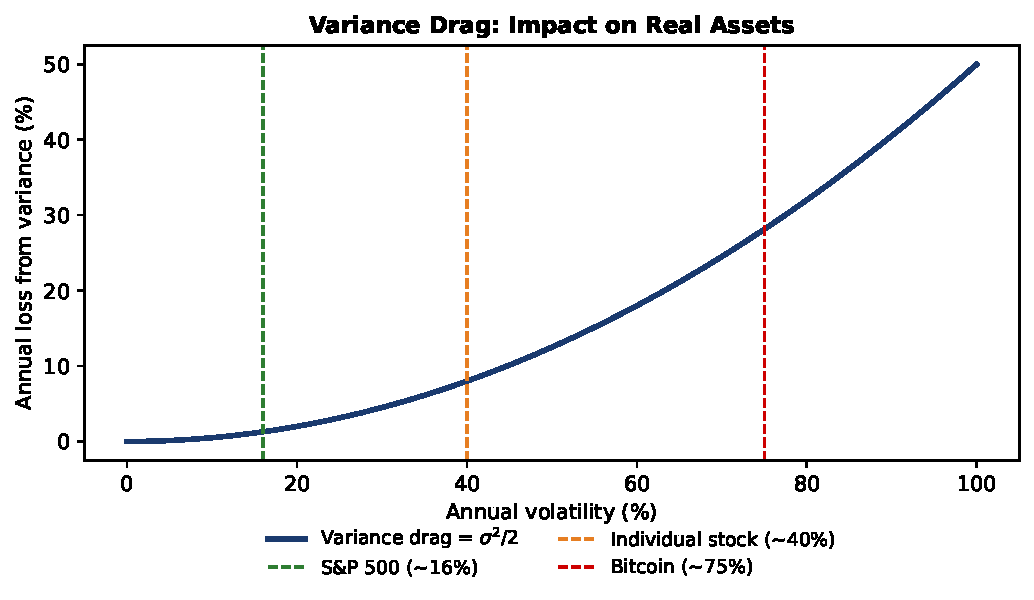
\includegraphics[width=0.58\linewidth]{sfm_ch1_variance_drag.pdf}
\end{center}
\vspace{-0.4cm}
\begin{itemize}
    \item \textbf{S\&P 500} ($\sigma \approx 16\%$): pierdere din varianță $\approx 1.3\%$/an --- neglijabilă
    \item \textbf{Acțiuni individuale} ($\sigma \approx 30\text{--}40\%$): pierdere $4\text{--}8\%$/an --- semnificativă
    \item \textbf{Bitcoin} ($\sigma \approx 75\%$): pierdere $\approx 28\%$/an --- devastatoare pe termen lung
    \item \textbf{Concluzie}: diversificarea reduce $\sigma$ și astfel reduce variance drag
\end{itemize}
\quantlet{SFM\_ch1\_variance\_drag}{https://github.com/QuantLet/Stat_fin_markets/tree/master/Ch_01/SFM_ch1_variance_drag}
\end{frame}

\begin{frame}[shrink=3]{Studiu de caz: S\&P 500 --- Distribuția empirică vs.\ Normala}
\begin{columns}[T]
\begin{column}{0.55\textwidth}
\begin{center}
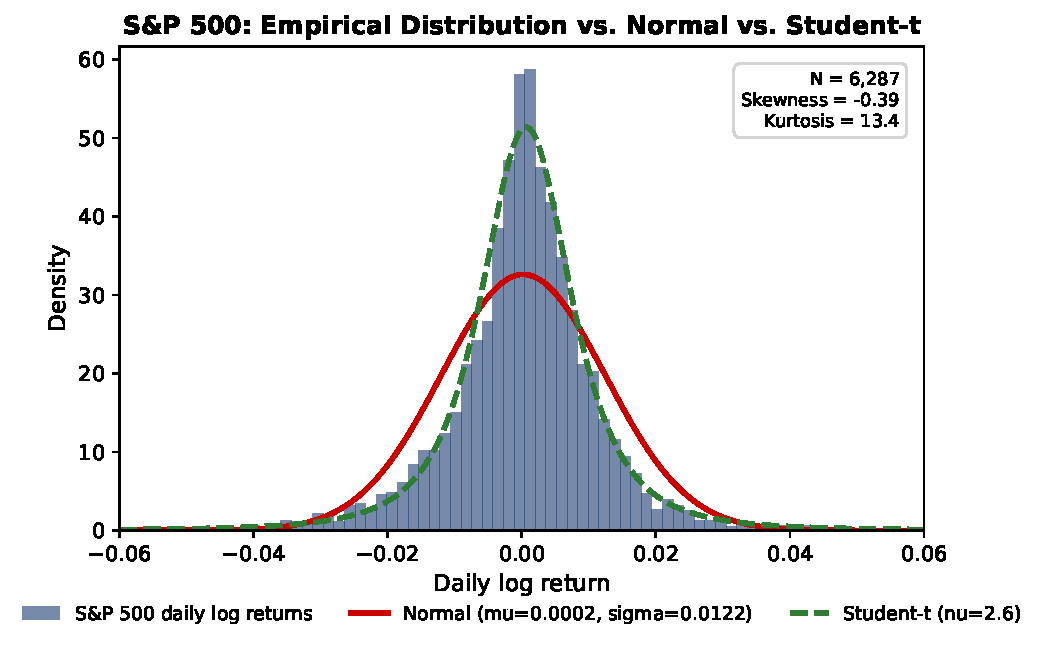
\includegraphics[width=\linewidth]{sfm_ch1_sp500_density.pdf}
\end{center}
\end{column}
\begin{column}{0.43\textwidth}
\begin{block}{Date reale: S\&P 500 (2000--2024)}
\begin{itemize}
    \item $N = 6\,287$ randamente zilnice logaritmice
    \item Histograma empirică vs.\ curba Normală vs.\ Student-$t$
\end{itemize}
\end{block}
\vspace{0.05cm}
\begin{alertblock}{Ce observăm?}
\begin{itemize}
    \item Vârful central \textbf{mai ascuțit} decât Normala
    \item Cozile \textbf{mai groase} --- crahuri mult mai frecvente
    \item $S = -0.39$, $K = 13.4$ (Normal: $S=0$, $K=3$)
    \item Student-$t$ cu $\nu \approx 3$ aproximează mai bine
\end{itemize}
\end{alertblock}
\end{column}
\end{columns}
\quantlet{SFM\_ch1\_returns\_analysis}{https://github.com/QuantLet/Stat_fin_markets/tree/master/Ch_01/SFM_ch1_returns_analysis}
\end{frame}

\begin{frame}[shrink=3]{Studiu de caz: QQ-Plot --- Verificare vizuală a normalității}
\begin{columns}[T]
\begin{column}{0.50\textwidth}
\begin{center}
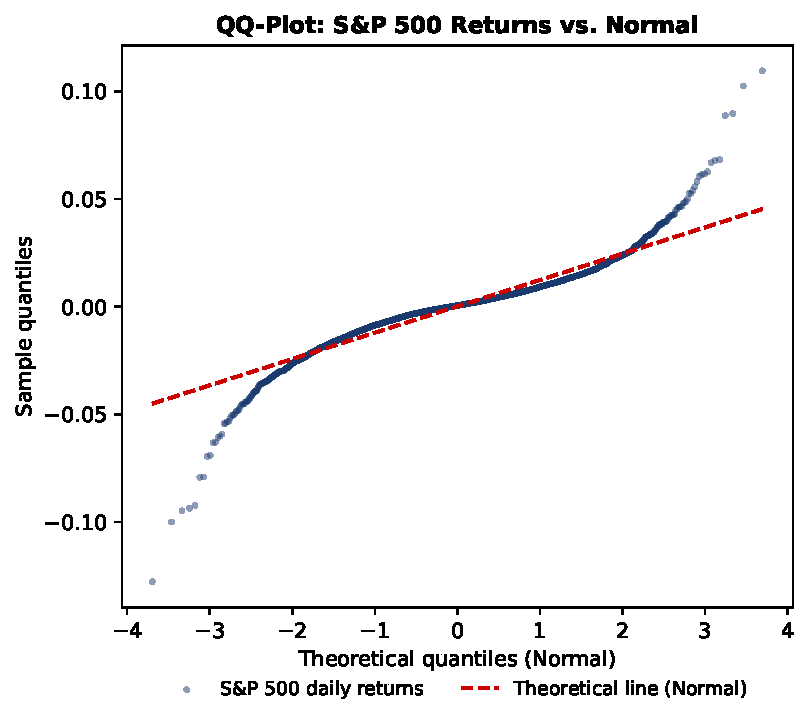
\includegraphics[width=\linewidth]{sfm_ch1_qqplot.pdf}
\end{center}
\end{column}
\begin{column}{0.48\textwidth}
\begin{block}{Cum citim un QQ-plot?}
\begin{itemize}
    \item Cuantilele eșantionului vs.\ cuantilele distribuției Normale
    \item Dacă datele sunt Normale $\Rightarrow$ punctele cad pe linia de $45^\circ$
\end{itemize}
\end{block}
\vspace{0.05cm}
\begin{alertblock}{Ce observăm?}
\begin{itemize}
    \item \textbf{Formă de S}: cozile deviază de la linie
    \begin{itemize}
        \item Coada stângă: pierderi mai extreme decât prevede Normala
        \item Coada dreaptă: câștiguri mai extreme
    \end{itemize}
    \item Testul Jarque-Bera confirmă formal:
    \begin{itemize}
        \item $JB = \frac{n}{6}\bigl(S^2 + \frac{\kappa^2}{4}\bigr) \sim \chi^2_2$
    \end{itemize}
\end{itemize}
\end{alertblock}
\end{column}
\end{columns}
\quantlet{SFM\_ch1\_stylized\_facts}{https://github.com/QuantLet/Stat_fin_markets/tree/master/Ch_01/SFM_ch1_stylized_facts}
\end{frame}

\begin{frame}[shrink=10]{Studiu de caz: Testul Jarque-Bera --- Respingerea formală a normalității}
\begin{defn}[Statistica Jarque-Bera]
\begin{itemize}
    \item $H_0$: $r_t \sim \mathcal{N}(\mu, \sigma^2)$
    \item $JB = \dfrac{n}{6}\!\left(S^2 + \dfrac{(K-3)^2}{4}\right) \;\xrightarrow{d}\; \chi^2_2$
    \item $S$ = skewness, $K$ = kurtosis, $n$ = dimensiune eșantion
\end{itemize}
\end{defn}
\begin{exampleblock}{Calcul pe S\&P 500 (2000--2024, $n = 6\,287$)}
\begin{itemize}
    \item $JB = \frac{6287}{6}\bigl((-0.39)^2 + (13.4 - 3)^2/4\bigr) = 1047.8 \times 27.19 = \mathbf{28\,488}$
\end{itemize}
\end{exampleblock}
\begin{center}
{\small\renewcommand{\arraystretch}{1.15}
\begin{tabular}{lccccc}
\toprule
\textbf{Activ} & $n$ & $S$ & $K$ & \textbf{JB} & $p$\textbf{-value} \\
\midrule
S\&P 500 & 6\,287 & $-0.39$ & $13.4$ & 28\,488 & $< 10^{-16}$ \\
AAPL     & 2\,516 & $-0.31$ & $8.6$  & 3\,168  & $< 10^{-16}$ \\
Bitcoin  & 3\,287 & $-0.15$ & $7.4$  & 2\,675  & $< 10^{-16}$ \\
\bottomrule
\end{tabular}}
\end{center}
\begin{itemize}
    \item Valoare critică: $\chi^2_{2, 0.01} = 9.21$
    \item Toate $JB \gg 9.21$ $\Rightarrow$ respingem $H_0$ la \textbf{orice} nivel de semnificație
\end{itemize}
\end{frame}

\begin{frame}[shrink=5]{Studiu de caz: Probabilitatea valorilor extreme}
\begin{block}{Cât de probabile sunt crahurile sub ipoteza de normalitate?}
\begin{itemize}
    \item Sub $\mathcal{N}(\mu,\sigma^2)$, un eveniment de $5\sigma$ are prob.\ $\approx 2.87 \times 10^{-7}$
    \item \textbf{Black Monday} (19 oct.\ 1987): S\&P 500 $-22.6\%$ într-o zi ($> 20\sigma$)
\end{itemize}
\end{block}
\vspace{0.1cm}
\begin{center}
{\small
\renewcommand{\arraystretch}{1.3}
\begin{tabular}{lcc}
\toprule
\textbf{Magnitudine} & \textbf{Prob.\ Normală} & \textbf{Frecvență observată} \\
\midrule
Mișcare $> 3\sigma$ & 0.27\% (1 la 370 zile) & $\sim$1 la 50--100 zile \\
Mișcare $> 4\sigma$ & 0.006\% (1 la 16\,000 zile) & $\sim$1 la 500--1000 zile \\
Mișcare $> 5\sigma$ & 1 la 3.5 mil.\ zile & $\sim$1 la 5000--10\,000 zile \\
\bottomrule
\end{tabular}
}
\end{center}
\vspace{0.1cm}
\begin{columns}[T]
\begin{column}{0.48\textwidth}
\begin{alertblock}{Concluzie}
\begin{itemize}
    \item Randamentele sunt \textbf{leptokurtice}
    \item Distribuția Normală subestimează dramatic riscul de coadă
\end{itemize}
\end{alertblock}
\end{column}
\begin{column}{0.48\textwidth}
\begin{exampleblock}{Implicație practică}
\begin{itemize}
    \item VaR sub normalitate \textbf{subestimează} pierderile extreme
    \item Empiric $\approx$ Student-$t$ cu $\nu \in [4,8]$
\end{itemize}
\end{exampleblock}
\end{column}
\end{columns}
\end{frame}

\begin{frame}{Studiu de caz: Momente empirice --- Comparație între active}
\begin{itemize}
    \item Statistici eșantion pentru randamente logaritmice zilnice, S\&P 500 (2000--2024), restul (2015--2024):
\end{itemize}
\vspace{0.1cm}
\begin{center}
{\small
\renewcommand{\arraystretch}{1.3}
\begin{tabular}{lcccccc}
\toprule
\textbf{Activ} & \textbf{Medie} & \textbf{Std} & \textbf{Skewness} & \textbf{Kurtosis} & \textbf{Min} & \textbf{Max} \\
\midrule
S\&P 500 & $+0.040\%$ & $1.00\%$ & $-0.39$ & $13.4$ & $-12.8\%$ & $+9.4\%$ \\
AAPL     & $+0.058\%$ & $1.80\%$ & $-0.31$ & $8.6$  & $-13.0\%$ & $+11.9\%$ \\
Bitcoin  & $+0.195\%$ & $3.90\%$ & $-0.15$ & $7.4$  & $-46.5\%$ & $+22.5\%$ \\
EUR/USD  & $+0.000\%$ & $0.45\%$ & $+0.08$ & $5.2$  & $-2.7\%$  & $+3.1\%$ \\
\bottomrule
\end{tabular}
}
\end{center}
\vspace{0.1cm}
\begin{itemize}
    \item Toate activele: excess kurtosis $\gg 0$ $\Rightarrow$ cozi groase (fat tails) confirmate
    \item Acțiuni și indici: skewness negativ $\Rightarrow$ riscul de crah domină
    \item Bitcoin: volatilitate maximă ($\sigma = 3.9\%$ zilnic $\approx 62\%$ anual)
    \item EUR/USD: medie $\approx 0$, aproape simetrică, dar cozi groase
\end{itemize}
\quantlet{SFM\_ch1\_returns}{https://github.com/QuantLet/Stat_fin_markets/tree/master/Ch_01/SFM_ch1_returns}
\end{frame}

%=============================================================================
% TEMĂ PENTRU ACASĂ
%=============================================================================
\section{Temă pentru acasă}

\begin{frame}[shrink=5]{Temă pentru acasă: Seminar 1}
\begin{block}{Analiza unei acțiuni românești (BVB)}
Alegeți o acțiune listată la Bursa de Valori București (ex.: TLV, SNP, BRD, FP, SNG). Perioadă: min.\ 3 ani.
\end{block}
\vspace{0.1cm}
\begin{columns}[T]
\begin{column}{0.48\textwidth}
\begin{exampleblock}{Cerințe de calcul}
\begin{enumerate}
    \item Randamente log zilnice (grafic)
    \item Statistici descriptive: $\hat\mu$, $\hat\sigma$, $S$, $K$
    \item Volatilitatea anualizată ($\times \sqrt{252}$)
    \item \textbf{Testul ADF} pe log-prețuri și pe randamente (raportați statistica, $p$-value, concluzie)
    \item \textbf{Testul Jarque-Bera}: calculați $JB$, raportați $p$-value, interpretați
\end{enumerate}
\end{exampleblock}
\end{column}
\begin{column}{0.48\textwidth}
\begin{block}{Cerințe de interpretare}
\begin{itemize}
    \item Sunt randamentele staționare? (ADF)
    \item Sunt normal distribuite? (JB)
    \item Comparați $\sigma$ cu S\&P 500 ($\approx 16\%$ anual)
    \item Calculați variance drag-ul --- e semnificativ?
\end{itemize}
\end{block}
\vspace{0.05cm}
\begin{alertblock}{Termen}
\begin{itemize}
    \item Următorul seminar
    \item Cod Python + grafice + 1 pagină interpretare
\end{itemize}
\end{alertblock}
\end{column}
\end{columns}
\end{frame}

%=============================================================================
% CE TREBUIE SĂ ȘTIE LA FINAL
%=============================================================================
\section{Rezumat}

\begin{frame}{Ce trebuie să știți la finalul Seminarului 1}
\begin{block}{Checklist de competențe}
\begin{enumerate}
    \item[\checkmark] \textbf{Diferența simplu vs.\ log}: simple sunt multiplicative, log sunt aditive temporal
    \item[\checkmark] \textbf{Compunerea randamentelor}: $1 + R_{\text{total}} = \prod(1+R_t)$ vs.\ $r_{\text{total}} = \sum r_t$
    \item[\checkmark] \textbf{Variance drag}: $\E[r] \approx \E[R] - \sigma^2/2$; volatilitatea distruge averea
    \item[\checkmark] \textbf{Motivul staționarității}: $P_t \sim I(1)$, $r_t \sim I(0)$; metodele statistice cer staționaritate
    \item[\checkmark] \textbf{Implementare Python}: descărcare date, calcul $r_t$, grafice preț vs.\ randamente
\end{enumerate}
\end{block}
\vspace{0.2cm}
\begin{exampleblock}{Nivel cognitiv atins}
\begin{columns}[T]
\begin{column}{0.48\textwidth}
\begin{itemize}
    \item Calcul operațional (manual + cod)
    \item Interpretare economică
\end{itemize}
\end{column}
\begin{column}{0.48\textwidth}
\begin{itemize}
    \item Legătura matematică--finanțe
    \item Început de gândire critică
\end{itemize}
\end{column}
\end{columns}
\end{exampleblock}
\end{frame}

%=============================================================================
% PLANIFICAREA COMPLETĂ A SEMINARELOR (4 SĂPTĂMÂNI)
%=============================================================================
\section{Planificarea seminarelor}

\begin{frame}{Structura seminarelor --- Capitolul 1 (4 săptămâni)}
\begin{center}
{\small
\renewcommand{\arraystretch}{1.4}
\begin{tabular}{>{\bfseries}clll}
\toprule
\textbf{Sem.} & \textbf{Tema} & \textbf{Conținut} & \textbf{Temă} \\
\midrule
1 & Randamente și staționaritate & Calcul $R_t$, $r_t$; variance drag; & Analiză acțiune \\
  & (acest seminar) & $I(1)$ vs $I(0)$; Python intro & BVB: randamente \\
\midrule
2 & Volatilitate & CC, rolling vol, $\sqrt{T}$; & Volatilitate 30z \\
  & & EWMA; comparație 20 vs 60z & pentru acțiune BVB \\
\midrule
3 & Fapte stilizate & Skew, kurtosis, QQ-plot; & Jarque-Bera test; \\
  & & ACF($|r_t|$); normalitate & verificare normalitate \\
\midrule
4 & Performanță și risc & Sharpe, MDD, Sortino; & Mini-proiect: \\
  & & mini-proiect complet & analiză completă \\
\bottomrule
\end{tabular}
}
\end{center}
\end{frame}


%=============================================================================
% TEST RAPID
%=============================================================================
\section{Test rapid}

\begin{frame}[shrink=3]{Test rapid --- Seminar 1 (15 minute)}
\begin{cminipage}{0.95\textwidth}
\begin{alertblock}{Răspundeți pe foaie (fără note)}
\begin{enumerate}
    \item Scrieți cele \textbf{3 condiții} ale staționarității slabe (covariance stationarity).
    \vspace{0.08cm}
    \item De ce ACF($r_t$) $\approx 0$ dar ACF($r_t^2$) $\neq 0$? Ce model motivează acest fapt?
    \vspace{0.08cm}
    \item Un activ are $\E[R] = 10\%$, $\sigma = 40\%$. Calculați variance drag-ul și averea după 20 de ani ($W_0 = 1$). Interpretați.
    \vspace{0.08cm}
    \item Un $R^2 = 0.92$ între prețul acțiunii A și prețul acțiunii B indică neapărat o relație reală? Argumentați.
    \vspace{0.08cm}
    \item Pentru un eșantion cu $n = 1000$, $S = -0.5$, $K = 8$, calculați statistica Jarque-Bera și concluzionați.
\end{enumerate}
\end{alertblock}
\end{cminipage}
\end{frame}

\begin{frame}[shrink=5]{Test rapid --- Răspunsuri}
\begin{cminipage}{0.95\textwidth}
\begin{exampleblock}{Răspunsuri}
\begin{enumerate}
    \item $\E[X_t] = \mu$; \; $\Var(X_t) = \sigma^2 < \infty$; \; $\Cov(X_t, X_{t+h}) = \gamma(h)$ --- primele două momente constante, autocovarianța depinde doar de lag-ul $h$.
    \vspace{0.05cm}
    \item Randamentele sunt necorelate (EMH) dar \textbf{nu independente}: magnitudinea lor este autocorelată. ACF($r_t^2$) captează \textbf{volatility clustering} $\Rightarrow$ motivație GARCH.
    \vspace{0.05cm}
    \item Drag $= \sigma^2/2 = 0.40^2/2 = 8\%$/an. $\E[r] = 10\% - 8\% = 2\%$/an. $W_{20} = e^{20 \times 0.02} = 1.49$. Randamentul aritmetic de 10\% se ``topește'' la doar 2\% geometric --- volatilitatea extremă distruge averea.
    \vspace{0.05cm}
    \item \textbf{Nu.} Ambele prețuri pot fi $I(1)$ cu trenduri comune (spurious regression, Granger \& Newbold 1974). Trebuie testat pe randamente ($R^2$ scade dramatic) sau testat cointegrarea.
    \vspace{0.05cm}
    \item $JB = \frac{1000}{6}((-0.5)^2 + (8-3)^2/4) = 166.7 \times (0.25 + 6.25) = \mathbf{1083.3}$. $\chi^2_{2, 0.01} = 9.21$. $1083.3 \gg 9.21$ $\Rightarrow$ respingem $H_0$ de normalitate.
\end{enumerate}
\end{exampleblock}
\end{cminipage}
\end{frame}

%=============================================================================
% BIBLIOGRAFIE
%=============================================================================
\section{Bibliografie}

\begin{frame}{Bibliografie și resurse}
\begin{cminipage}{0.95\textwidth}
\begin{block}{Referințe cheie}
    {\small
    \begin{itemize}\setlength{\itemsep}{1pt}
        \item Franke, J., Härdle, W.K., Hafner, C.M. (2019). \textit{Statistics of Financial Markets}. 4th Ed., Springer.
        \item Cont, R. (2001). Empirical Properties of Asset Returns. \textit{Quantitative Finance}, 1(2), 223--236.
        \item Dickey, D.A., Fuller, W.A. (1979). Distribution of the Estimators for AR Time Series with a Unit Root. \textit{JASA}, 74, 427--431.
        \item Granger, C.W.J., Newbold, P. (1974). Spurious Regressions in Econometrics. \textit{J.\ of Econometrics}, 2(2), 111--120.
        \item Mandelbrot, B. (1963). The Variation of Certain Speculative Prices. \textit{J.\ of Business}, 36(4), 394--419.
    \end{itemize}
    }
\end{block}
\vspace{0.1cm}
\begin{exampleblock}{Resurse online}
    {\small
    \begin{itemize}\setlength{\itemsep}{1pt}
        \item \textbf{GitHub}: \url{https://github.com/QuantLet/Stat_fin_markets} --- cod Python complet
        \item \textbf{Quantlet}: \url{https://quantlet.com} \hspace{0.3cm} \textbf{Quantinar}: \url{https://quantinar.com}
    \end{itemize}
    }
\end{exampleblock}
\end{cminipage}
\end{frame}

%=============================================================================
% MULȚUMESC
%=============================================================================
{
\setbeamertemplate{headline}{}
\setbeamertemplate{footline}{}
\begin{frame}{}
    \centering
    \Huge\textcolor{MainBlue}{Vă mulțumesc!}

    \vspace{0.8cm}

    \Large Întrebări?

    \vspace{1cm}

    \normalsize
    Materialele cursului disponibile la: \url{https://danpele.github.io/SFM/}

    \vspace{0.3cm}

    \href{https://quantlet.com}{\raisebox{-0.15em}{
\includegraphics[height=0.8em]{ql_logo.png}} Quantlet} \hspace{0.5cm}
    \href{https://quantinar.com}{\raisebox{-0.15em}{
\includegraphics[height=0.8em]{qr_logo.png}} Quantinar}
\end{frame}
}

\end{document}
